% Chapter 1

\chapter{Introducción} % Chapter title

\label{ch:introduccion} % For referencing the chapter elsewhere, use \autoref{ch:introduccion}
\lhead{\emph{Introducción}} % Change X to a consecutive number; this is for the header on each page - perhaps a shortened title

%----------------------------------------------------------------------------------------
En esta capítulo se introduce brevemente la problemática a resolver asi como la estructura de la tesis.

En la Sección \ref{sc:definitions} se introducen la definiciones previas, necesarias, para el desarrollo de la tesis, utilizadas
luego como conocimientos de base, necesarias para poder comprender el trabajo en su totalidad.

En la Sección \ref{sc:context} se introduce el contexto del problema, para poder comprender el marco de área de estudio
propuesto, el tipo de antena objeto de estudio, los tipos de calibración y la importancia de la calibración interna.

En la Sección \ref{sc:motivation} se introduce cual es la motivación para la realización de la presente tesis. Se hace foco
en la calibración interna, sus virtudes y defectos y la necesidad de resolver problemas que la calibración clásica no resuelve.
Existen diversos métodos pero en todos se propone la incorporación de HW externo adicional lo cual en algunos casos puede ser
no implementable.

En la Sección \ref{sc:objective} se introduce el Objeto de la Tesis. Se propone un método para complementar al método clásico
de calibración interna sin necesidad de tener que agregar HW externo. Se proponen todos los puntos a desarrollar a lo largo de
esta tesis. Por ejemplo, el desarrollo de un modelo de base en RF sobre el cual probar la propuesta.

En la Sección \ref{sc:specifications} se introducen las Especificaciones del Problema. Es decir, las hipótesis de base que se
toman como necesarias para poder implementar el método propuesto.

En la Sección \ref{sc:methodology}, se explica la metodología utilizada a lo largo del proceso de desarrollo de la tesis.

En la sección \ref{sc:contribution} se introduce la contribución del presente trabajo de tesis a la comunidad científica.

En la sección \ref{sc:structure}, se introduce la Estructura de la tesis, en donde se detallan los capítulos de la tesis y su
contenido.


\section{Definiciones previas} \label{sc:definitions}

A continuación se introducen algunas definiciones previas necesarias para el desarrollo de la tesis.


{\textbf{Antena:}} Es definida como la estructura transicional enre espacio libre y un dispositivo guía, como se muestra en la 
figura \ref{fig:antenna}. El dispositivo guía o línea de transmisión puede ser un cable coaxial o un tubo hueco (guía de 
onda), el cual es utilizado para transportar energía electromagnética desde la fuente de transmisión a la antena, o deade la 
antena al receptor. En el primer caso sería una configuración de antena transmisora y en el segundo, receptora \cite{Balanis2012}.
\begin{figure}[H]
 \centering
 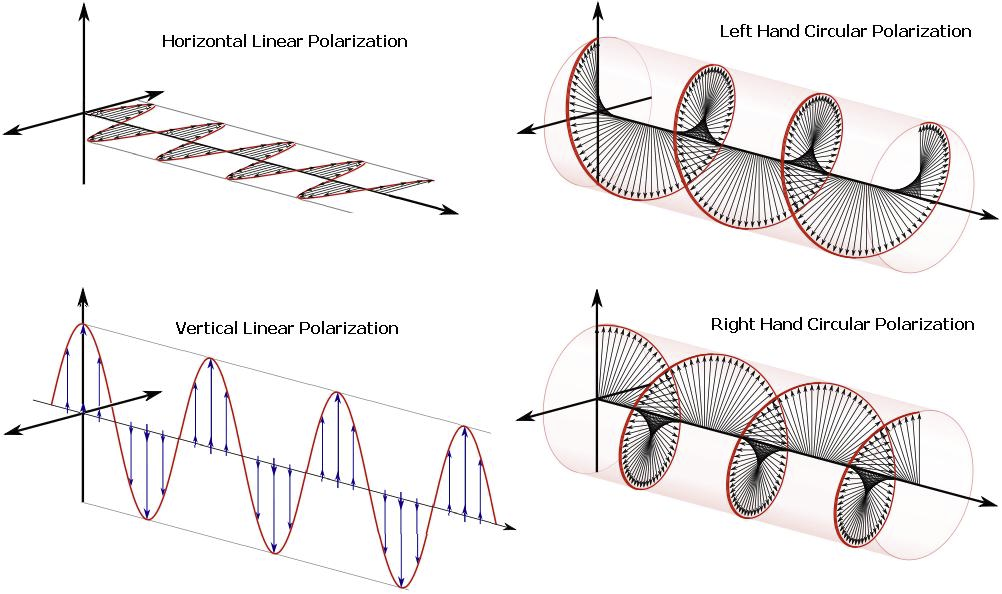
\includegraphics[width=10cm]{gfx/polarizations.png}
 \caption{Antena como un dispositivo de transmisión \cite{Balanis2012}}
 \label{fig:antenna}
\end{figure}

{\textbf{Polarización:}} La polarización de una onda de radio en general hace referencia a la orientación del campo
eléctrico (plano-E) de la onda de radio con respecto a la superficie terrestre (ver figura \ref{fig:hvPolarizations}). La antena
que la genera determina, de acuerdo con su estructura física y orientación, qué tipo de polarización tendrá la onda emitida.
Por dar un ejemplo, una antena que sea simplemente un cable recto poseerá una polarización cuando se la monta verticalmente, y
otra diferente cuando sea horizontalmente. Como una onda transversal, el campo magnético de una onda de radio es perpendicular
al eléctrico en campo lejano, pero, por convención, la polarización hace referencia a la dirección del campo eléctrico
\cite{AntennaWiki}.

\begin{figure}[H]
 \centering
 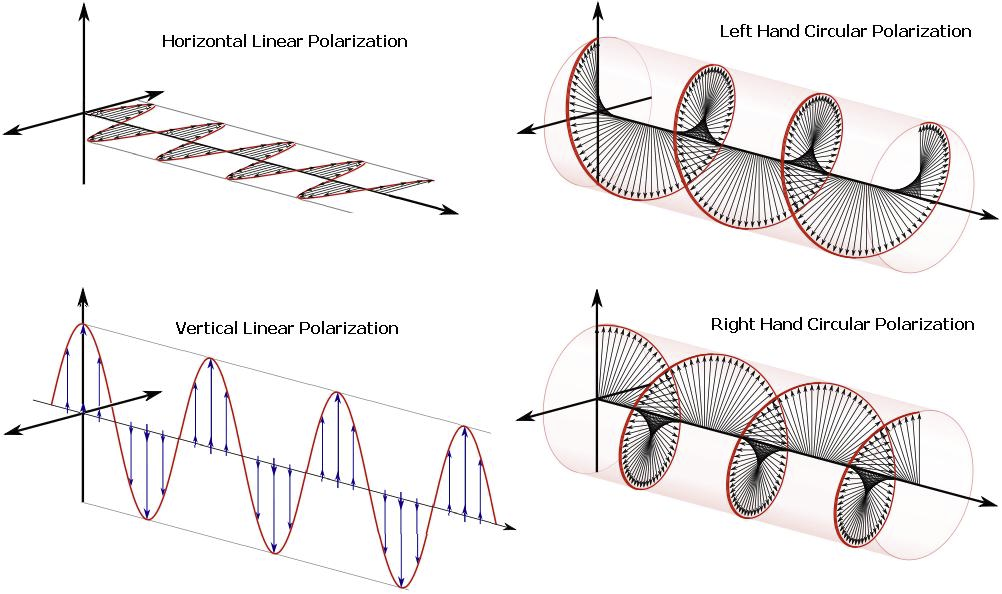
\includegraphics[width=10cm]{gfx/polarizations.png}
 \caption{Distintos tipos de polarizaciones \cite{polarization}}
 \label{fig:hvPolarizations}
\end{figure}

{\textbf{Diagrama de radiación:}} Es la representación gráfica de la densidad de potencia de las ondas radiadas por la antena
en función del ángulo. Típicamente se lo representa en un gráfico de tres dimensiones o en diagramas de dos dimensiones de
cortes transversales horizontales y verticales \cite{AntennaWiki}.

\begin{figure}[H]
 \centering
 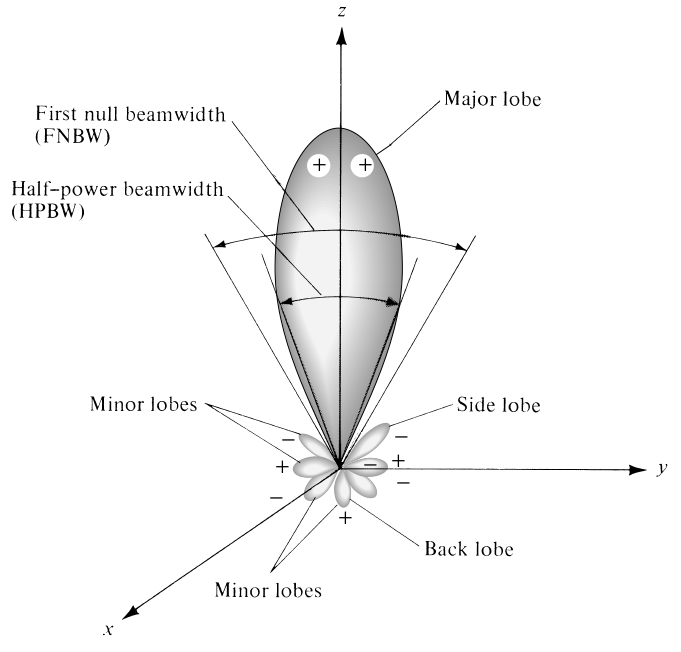
\includegraphics[width=10cm]{gfx/arrayPattern.png}
 \caption{Ejemplo de diagrama de radiación \cite{diagramaRadiacion}.}
\end{figure}

{\textbf{Apuntamiento del haz:}} Es cambiar la dirección del lóbulo principal de un diagrama de radiación \cite{BeamSteering}.

{\textbf{Huella:}} Es el área terrestre visible para el satélite \cite{Footprint}. 

{\textbf{VNA:}} Un VNA es un instrumento que mide los parámetros eléctricos de una red. Hoy, dichos analizadores miden los 
parámetros S porque las reflexiones y transmisiones de redes eléctricas son fácilmente medibles en alta frecuencia. Normalmente
caracterizan redes de dos puertos \cite{NetworkAnalyzer}.

{\textbf{Directividad:}} Es una figura de mérito de una antena. Es el cociente entre la densidad de potencia radiada en la
dirección de máxima emisión y la densidad de potencia radiada utilizando un radiador isotrópico (el cual emite uniformemente
en toda dirección) \cite{DirectivityWiki}.

{\textbf{SWR o ROE:}} Es una medida de adaptación entre la carga y la impedancia característica de una línea de transmisión. Las
desadaptaciones de impedancias resultan en ondas estacionarias a lo largo de dicha línea de transmisión. El SWR está
definido como la relación entre la amplitud de la onda reflejada y la amplitud de la onda incidente \cite{swrWiki}.

{\textbf{Adaptación de impedancias:}} La máxima transferencia de potencia requiere que la impedancia de un sistema de
antena esté adaptada al complejo conjugado de la impedancia del transmisor o receptor. En el caso de un transmisor,
la impedancia adaptada deseada no necesariamente corresponde a la impedancia de salida dinámica del transmisor analizado
como una impedancia sino al valor de diseño (típicamente de $50 \Omega$) requerido para una operación eficiente
y segura del circuito de transmisión. Normalmente, la impedancia deseada es resistiva pero un transmisor (y algunos receptores)
pueden tener ajustes adicionales para cancelar una cierta cantidad de reactancia en orden de obtener dicha adaptación. Cuando
una linea de transmisión es utilizada entre la antena y el transmisor (o receptor) uno generalmente desearía un sistema de antena
con una impedancia resistiva cercana a la impedancia característica de dicha línea de transmisión, para minimizar el SWR
e incrementar la transmisión \cite{AntennaWiki}.

{\textbf{Conjunto de Antena con fase variable (en inglés: Phased Array):}} es un conjunto de antenas en que las fases relativas
de las señales con que se alimenta cada antena se varían intencionadamente con objeto de alterar el diagrama de radiación del
conjunto. Lo normal es reforzar la radiación en una dirección concreta y suprimirla en direcciones indeseadas. Si todos los
elementos del conjunto están contenidos en el mismo plano y la señal con que se alimentan es de la misma fase,
entonces se estará reforzando la dirección perpendicular a ese plano. Si se altera la fase relativa de las señales se podrá
\enquote*{mover} el haz (en realidad lo que se está haciendo es cambiar la dirección en la cual las interferencias son
constructivas). Se consigue de este modo hacer barridos sin necesidad de movimiento físico, con la ventaja añadida de que
se pueden barrer ángulos del orden de miles de grados por segundo. Esto permite utilizar la antena para compaginar
simultáneamente funciones de detección y de seguimiento muchos blancos individuales, así como para obtener imágenes de
apertura sintética. Su uso se va extendiendo debido a la confiabilidad derivada del hecho de que no tienen partes móviles.
Casi todos los radares militares modernos se basan en phased arrays, relegando los sistemas basados en antenas rotatorias a
aplicaciones donde el costo es un factor determinante (tráfico aéreo, meteorología, etc) Su uso está también extendido en
aeronaves militares debido a su capacidad de seguir múltiples objetivos. El primer avión en usar uno fue el B-1B Lancer, y
el primer caza, el MiG-31 ruso.\\

{\textbf{Calibración:}} Operación que, bajo determinadas condiciones, en un primer paso, establece una relación entre
valores cuantitativos con incertidumbres de medición provistas por estándares de medición e indicaciones correspondientes
con incertidumbres asociadas (del instrumento calibrado o estándar secundario) y, en un segundo paso, usa
esta información para establecer una relación para obtener un resultado de una medición desde una indicación \cite{CalDef}.

{\textbf{Calibración interna:}} Las mediciones obtenidas utilizando este sistema son útiles solamente al utilizarlas en
conjunto a los resultados de los test realizados en tierra, los cuales definen la relación entre lo observado y la
performance de los parámetros del sistema. Ejemplos de satélites para los cuales se utilizó calibración interna son el
E-ERS-1 y el SIR-C.

Los tests realizados en tierra para dichos sistemas complejos son sobre la electrónica de RF, la electrónica digital y la
antena sobre temperatura; para los cuales es preferible realizarlos, cuando sea posible, en un ambiente al vacío. Los
parámetros clave del sistema, como: potencia transmitida, pérdidas de transmisión o recepción, ganancia de recepción,
ganancia y diagrama de radiación de la antena, linealidad de la electrónica digital/RF, rango dinámico, y fase/amplitud vs
estabilidad de la frecuencia son medidos en función de la temperatura para cada configuración de ganancia del radar y PRF. Los elementos de calibración, como medidores de temperatura, de corriente y de potencia, podrán
permitir la determinación dela modela en RF. la performance del sistema en función de la variación de dichos parámetros.

Esta técnica asume que la variación en la performance del sistema puede ser modelada en función de los parámetros observables.
También, se asume que los componentes de calibración están correctamente calibrados y son estables en el paso del tiempo.
Además de estos tests, en la mayoría de los sistemas de radar se realizan mediciones de componentes de RF utilizando lazos de
calibración \cite{Curlander1991}.

{\textbf{Caracterización:}} significa medir (el desempeño de) los parámetros de la antena con el objeto de describir en
forma comprensible su comportamiento \cite{Mittermayer2007}.

{\textbf{Caracterización del sistema:}} adicionalmente incluye la determinación de las curvas de características basadas
en los modelos y en las mediciones indirectas de los parámetros, en el caso en que los parámetros no pueden ser medidos
en forma directa \cite{Mittermayer2007}.

{\textbf{Calibración:}} significa el ajuste de la representación de los parámetros físicos en los productos que arroje la
antena de manera que los mismos puedan ser medidos dentro la especificación \cite{Mittermayer2007}.

{\textbf{Verificación:}} significa mostrar mediante mediciones apropiadas que un sistema o subsistema trabaja dentro de su
especificación (o conjunto de especificaciones) o que un producto cumple con su especificación \cite{Mittermayer2007}.

\section{Contexto} \label{sc:context}

Una antena es un transductor que transforma la energía eléctrica conducida en energía electromagnética radiada cuando
trabaja como transmisora, o viceversa cuando actúa como receptora.

Hay una amplia variedad de antenas en la actualidad, se realiza una agrupación simplificada en la tabla \ref{tab:type_antennas}.

\begin{table}[H]
  \footnotesize
  \centering
  \begin{tabular}{|c|p{9cm}|}
	\hline
	\textbf{Tipo Antena} & \textbf{Características} \\\hline
	Isotrópica & Es una antena hipotética, la cual radia la misma potencia en todas las direcciones.\\\hline
	Monopolo & Es un único módulo radiante, generalmente un simple cilindro de metal conectado en una punta a un plano de
	tierra y en la otra a la línea de alimentación. Usos: Radio AM/FM, walkie talkie, etc. \\\hline
	Dipolo & Es el tipo de antena más comúnmente utilizada, consiste en dos RMs simétricos, los cuales son cilindros
	metálicos o cables. Usos: antena de canales de tv VHF, antena de televisión analógica, etc. \\\hline
	Conjunto & Consiste en múltiples antenas trabajando como una única antena. Usos: Transmisión de canales de tv en VHF,
	detección de misiles, comunicaciones satelitales, etc.\\\hline
	Lazo & Consiste en una o múltiples vueltas de cable. Trabajan con campos magnéticos en vez de eléctricos. Usos: receptora
	de canales UHF de tv, receptoras de radio de Amplitud Modulada, etc.\\\hline
	Apertura & Son el principal tipo de antenas direccionales utilizadas en frecuencias microondas. Consisten en una antena
	del tipo dipolo o Lazo junto a una estructura que guía las ondas en una dirección determinada. Usos: Comunicaciones
	satelitales, comunicaciones marinas, etc.\\\hline
  \end{tabular}
  \caption{Características de cada grupo principal de antenas}
  \label{tab:type_antennas}
\end{table}

La presente tesis se enfoca en el tipo \enquote*{conjunto de antena de fase controlada de manera electrónica}, en inglés
\enquote*{phase array electronically controlled antenna}. Este tipo de antenas son ampliamente utilizadas de manera masiva
en aplicaciones donde es necesario realizar apuntamientos en diferentes direcciones con altas velocidades. Por ejemplo,
comunicaciones móviles \cite{Chen2012}, aéreas \cite{MHong1989} y espaciales \cite{Shimada1995}\cite{Makhoul2012}. En el capítulo
\ref{ch:phasedArray} se explica el principio de funcionamiento básico de dicho tipo de antena.

Para generar diversos productos, por ejemplo imágenes satelitales en radares SAR \cite{Freeman1992}, es necesario que la
antena se encuentre correctamente calibrada \cite{Luscombe1990}\cite{Seifert1996}\cite{Dall1994}. Esto implica, que las
tolerancias de fase y amplitud se mantengan en el tiempo y/o sus valores sean bien conocidas para cada elemento del conjunto.

Un método de calibración en tierra para estas antenas es la de utilización de fuentes externas de campo lejano o cercano
\cite{Agrawal2003}. Sin embargo, en aplicaciones aéreas o espaciales, la utilización de dichas fuentes es impráctica o
difícil de implementar \cite{Aumann1989}. Para estos casos se utilizan esquemas de calibración externa e interna.

Hay dos grupos principales de calibración externa a saber,
\begin{itemize}
	\item Calibración utilizando blancos puntuales: Los blancos puntuales son dispositivos construidos por el hombre, generalmente
		corner reflectors, transponders, generadores de tono o receptores. La característica de estos dispositivos es que no
		solo son muy chicos con respecto a la mínima área de observación de una antena y que el eco de la señal de dichos
		dispositivos posee mucha más intensidad que dicha área, sino que el reflejo es bien conocido. Por lo tanto, con su uso
		se puede deducir la potencia transmitida.
	\item Calibración utilizando blancos distribuidos: Se refiere a la utilización de blancos naturales de largas áreas con
		propiedades de dispersión homogéneas. Se utiliza la suposición que dichas propiedades son estables o que su variación es
		bien conocida.
\end{itemize}

El mayor problema de dichos esquemas de calibración es que el tiempo de revisita a dichos lugares de calibración en tierra es muy
grande y solo se puede calibrar la ganancia absoluta del conjunto de antena en su totalidad. Para disminuir el tiempo entre
calibraciones y para poder calibrar cada elemento del conjunto de forma individual surge diversos esquemas de calibración
interna.

El primer método a mencionar es el llamado método REV, el cual calibra de a un módulo radiante a la vez utilizando una
antena externa al panel como receptora. En el proceso de calibración se transmite de a un módulo radiante a la vez
y se va variando su fase hasta obtener la máxima potencia recibida. Repitiéndose el proceso para todos los elementos.

Otro método es el convencional (descripto en el capítulo \ref{ch:classicalCalibration}), el cual implementa lazos internos
para calibrar los caminos de transmisión y recepción de la antena de forma independiente \cite{Makhoul2012}
\cite{Luscombe1990}\cite{Seifert1996}\cite{Dall1994}\cite{Freeman1995}\cite{Bibby2003}\cite{Bast2003}\cite{Stove2004}
\cite{Srivastava1996}\cite{Wang2010}. Para ello, la señal de calibración recibida se la compara con la potencia transmitida,
obteniendo así, que dicha diferencia se corresponde con el desfasaje de potencia y fase de cada camino de transmisión/
recepción. Luego, se opta por caracterizar todos aquellos componentes que no pertenecen a ningún lazo de calibración
\cite{Freeman1995}. Este método presenta algunos inconvenientes. Por dar un par de ejemplos se puede mencionar que los recursos
necesarios (tiempo, personal) durante la campaña de ensayos previa al lanzamiento impactan en todo el desarrollo de actividades,
o las consecuencias que puede traer el hecho que la caracterización no sea válida porque un determinado componente
envejece con el paso del tiempo.

En este contexto, se investiga y propone un método que permita reducir costos asociados a la calibración y por ende a los
proyectos:

\begin{enumerate}
    \item Evitando la necesidad de realizar caracterizaciones previas del conjunto de antena.
    \item Permitiendo conocer en tiempo real, y para el estado real de la antena, los valores reales de fase y amplitud en
		vuelo que transmite la antena, independientemente de su estado de envejecimiento.
\end{enumerate}

En este sentido se investiga y aprovecha el concepto acoplamiento mutuo inherente entre los módulos radiantes de la antena
\cite{Aumann1989}, pero de manera complementaria al enfoque tradicional. Este método calibra tanto los caminos de transmisión
como recepción a la vez, para ello, se transmite en una polarización y se recibe en otra de a un módulo radiante a la vez.
Una ventaja que tiene frente a los otros métodos realizados es que no solo calibra la antena en su totalidad, sino también
sirve para determinar si hay módulos radiantes en mal funcionamiento o directamente inhabilitados.

\section{Motivación} \label{sc:motivation}

Para poder hacer un uso adecuado del PA es necesario conocer la fase y atenuación de cada uno de los elementos del mismo, tanto
cuando transmiten como cuando recibe. Sin embargo, si bien uno controla la fase y atenuación de cada elemento, la RFDN no permite
necesariamente asegurar que la fase y atenuación con que sale la señal sea realmente la deseada. Hay fenómenos de dispersión en
la RFDN debidos a la temperatura que hacen que la fase deseada y la requerida sean diferentes \cite{Keizer2011}.

El método de calibración tradicional, por lazos de calibración internos, permite calibrar un conjunto de antena, aunque
adolece de algunos defectos entre los cuales se incluyen:

\begin{enumerate}
    \item Un mal funcionamiento o directamente la inhabilitación de un elemento radiante, el cual está fuera del lazo de
		calibración interno, no es detectado por la calibración interna.
    \item Existen elementos que quedan fuera del lazo de calibración interna. Como por ejemplo los circuladores. Esto lleva a
		la necesidad de realizar caracterizaciones en tierra, lo cual implica un consumo de recursos de proyecto importantes,
		además de tener que confiar que dicha caracterización será válida (o sea que no habrá envejecimiento de los mismo)
		durante toda la vida útil de la antena.
    \item Cada lazo de calibración no se interrelaciona con el resto haciendo que no se pueda disminuir el error de medición por
		multiplicidad de caminos.
\end{enumerate}

El conocimiento de dichas limitaciones llevan a investigar opciones superadoras, que den lugar a un método de calibración que 
permita ser complementario al tradicional. 
\begin{enumerate}
	\item Evitando la necesidad de realizar costosas caracterizaciones en tierra
	\item Previendo que los componentes en vuelo puedan envejecer y por ende modificar sus características.
	\item Permitiendo detectar fallas en elementos que en la calibración interna tradicional están fuera del lazo de calibración.
	\item Disminuyendo la incertidumbre en la determinación de la fase y amplitud de salida.
\end{enumerate}

El método proupesto en esta tesis, denominado de \enquote*{diseño y calibración de una antena polarimétrica por 
acoplamientos mutuos}, toma la idea de mediciones por acoplamiento mutuo \cite{Agrawal2003}\cite{Shipley2000} \cite{Aumann1989}
\cite{Chen2012} para integrarla de manera complementaria al método tradicional sin necesidad de agregar hardware adicional. 
Además, se establecen los requerimientos electrónicos para poder implementarla. Para poder comparar el comportamiento y 
eficiencia de ambos métodos, se realiza un modelo de antena polarimétrica.

\section{Objetivo de la Tesis} \label{sc:objective}

La presente tesis tiene varios objetivos:

\begin{enumerate}
    \item Presentar conceptualmente el método tradicional de calibración interna de una antena polarimétrica. Con sus 
		virtudes y defectos. Mencionar algunas misiones de ejemplo en las cuales el mismo se ha utilizado.
    \item Investigar, desarrollar y presentar conceptualmente un método alternativo de calibración interna que introduzca
		mejoras al método tradicional sin necesidad de introducir hardware adicional y con la premisa fundamental de
		reducir los costos asociados a las caracterizaciones que el método tradicional incluye. Introducir los
		requerimientos necesarios para poder implementarlo.
    \item Investigar e implementar el modelo de antena polarimétrico que será utilizado para poder comparar el 
		método tradicional y el alternativo. Dicho modelo debe representar el comportamiento en RF básico de las señales al 
		propagarse por el sistema.
    \item Implementar los sistemas de calibración tradicional y alternativo que actúen sobre el modelo de antena. 
    \item Sacar conclusiones respecto a los pros y contras del método propuesto, en particular en referencia al método
		tradicional, por medio de algunos parámetros objetivos como ser tiempo de calibración, caracterizaciones necesarias,
		incertidumbre de medición, entre otros.
\end{enumerate}


\section{Especificaciones del problema} \label{sc:specifications}

Para poder aplicar e implementar el método de acoplamientos mutuos se deben cumplir las siguientes hipótesis de base, que a su
vez son consideradas las especificaciones del problema.

\begin{enumerate}
    \item Modularización de los componentes de la antena: La antena debe estar compuesta por desfasadores, atenuadores, cables,
		divisores de potencia y elementos radiantes.

	\item Modelización de los componentes en RF: Los componentes de la antena deben caracterizarse utilizando parámetros de alta
		frecuencia.

    \item Sistemas LTI: La aplicación deberá reproducir el comportamiento del sistema, el cual será LTI (lineal e invariante
		en el tiempo).

	\item Adaptación de impedancias: Todos los componentes se encuentran perfectamente adaptados.

    \item Variabilidad para determinados componentes: Se deben poder utilizar distintos divisores/combinadores de potencia.
		La diferencia entre ellos es la cantidad de puertos de salida.

    \item Dimensión de antena: Se debe poder configurar la cantidad de elementos radiantes por columna y fila de la antena.
    \item Distancia entre elementos radiantes: Se debe poder configurar la distancia entre elementos radiantes.
    \item Configuración individual de componentes: Se debe poder configurar los atributos que afecten la modelización de cada
		componente de la antena. Largo, atenuación y desfasaje por metro de cables.

    \item Modelizaciones dispersiones: Se debe poder configurar la dispersión en el comportamiento de cada componente de la
		antena de forma independiente.

    \item Introducción de elementos de control en el lazo de calibración: Se deben poder configurar los atenuadores y
		defasadores a la hora de realizar la calibración.

    \item Calibración clásica: La aplicación debe poder calibrar una antena polarimétrica con el método de calibración convencional.

    \item Calibración alternativa: La aplicación debe poder calibrar una antena polarimétrica con el método de calibración alternativo.

    \item Calibración ganancia: La aplicación debe poder calibrar la ganancia de transmisión y recepción.

    \item Calibración fase: La aplicación debe poder calibrar la fase de transmisión y recepción.

    \item Cal. pol. horizontal: La aplicación debe poder calibrar en la polarización horizontal.
    \item Cal. pol. vertical: La aplicación debe poder calibrar en la polarización vertical.
    \item Cal. Tx: La aplicación debe poder calibrar en transmisión.
    \item Cal Rx: La aplicación debe poder calibrar en recepción.

    \item Calibración independiente del estado inicial: Se debe poder alcanzar el estado de calibración deseado partiendo
		cualquier estado inicial en los desfasadores y atenuadores.

    \item Transmisión vs recepción por polarizaciones cruzadas: Para calibrar se debe transmitir y recibir en polarizaciones
		diferentes.

    \item Planitud de antena: La antena tiene que ser perfectamente plana. No deben haber imperfecciones.

    \item Frecuencia de RF: Se debe poder configurar la frecuencia de trabajo.

    \item Dispersión señal de calibración entre pulsos: Se debe poder configurar los parámetros de dispersión (desvío estándar) para
		la ganancia y fase de la chirp utilizada entre pulsos.

    \item Dispersión chirp réplica: Se debe poder configurar los parámetros de dispersión (desvío estándar) para la
		ganancia y fase de la chirp réplica utilizada a la hora de realizar la calibración convencional.

    \item Dispersión walsh: Se debe poder configurar los parámetros de dispersión (desvío estándar) para la fase de la
		codificación utilizada a la hora de realizar la calibración convencional.

    \item Simulación falla componente: Se debe poder simular, configurar la destrucción total de los TRMs o RMs de la antena.
\end{enumerate}


\section{Metodología de la tesis} \label{sc:methodology}

En la presente tesis se investigan los métodos de calibraciones actuales determinando las ventajas, desventajas,
limitaciones y diferencias que hay entre cada una de ellos. De esta forma, se obtiene una visión global para
determinar las posibles falencias puede tener este método alternativo.

Posteriormente, se investigan las limitaciones que poseen las antenas polarimétricas para determinar que recaudos
se deben tener en cuenta a la hora de desarrollar el método.

Luego, tomando todo en cuenta, se determinan las hipótesis necesarias para que el algoritmo funcione correctamente. Para
la validación del método se realiza un modelo de antena.

Finalmente, se prueban, analizan y documentan los resultados obtenidos de la comparación entre el algoritmo propuesto
y el algoritmo de la calibración convencional. A su vez, se deja asentado que posibles mejoras se podrían aplicar al
algoritmo para determinar otros aspectos que están fuera del alcance de esta tesis.

\section{Contribución} \label{sc:contribution}

Como contribución se desarrolla un modelo de antena que cumple con todos los requerimientos del problema previamente
mencionados, logrando así, que sea representativo en RF. A su vez, dicho modelo puede ser reutilizado para modelar cualquier 
tipo de estrategia de calibración futura.

Además, este método de calibración aporta el hecho de poder calibrar no solo la potencia, sino que también la fase
manteniendo el apuntamiento en que se va a utilizar dicha antena.

Como punto final, se presenta la comparación del método alternativo con el clásico, mostrando las ventajas, desventajas y que
tan compatibles son entre ambos.


\section{Estructura de la Tesis} \label{sc:structure}

Los siguientes capítulos se organizan de la siguiente manera:

\begin{enumerate}
	\item Capítulo 2: Se presenta y detalla una antena polarimétrica, haciendo hincapié en el diagrama de radiación y como
    se realiza su modelización en RF.
	\item Capítulo 3: Se presenta y detalla el método de calibración clásica planteando sus ventajas y desventajas.
	\item Capítulo 4: Se presenta y detalla el método de calibración por acoplamientos mutuos planteando sus ventajas y
		desventajas.
	\item Capítulo 5: Se detalla la modelización y estructura del modelo de la antena implementado para realizar los ensayos.
	\item Capítulo 6: Se presentan los ensayos realizados sobre el modelo de antena utilizando distintos factores de errores y
		comparando los resultados obtenidos por ambos calibradores.
	\item Capítulo 7: Se presentan los resultados obtenidos, conclusiones y posibles trabajos futuros a realizar.
	\item Apéndices
\end{enumerate}

